\vspace{1.5pc}
\section[Domain Penelitian]{Domain Penelitian}
\begin{spacing}{1.5}
	Domain penelitian meliputi wilayah BoB, perairan Andaman, dan samudra Hindia dengan koordinat $5.5^\circ-24.6^\circ$ LU dan $78.2^\circ-96.7^\circ$ BT (lihat Gambar \ref{fig:domain}). Data batimetri untuk domain penelitian diperoleh dari SRTM15+ \href{https://topex.ucsd.edu/pub/archive/srtm15/V1/}{(https://topex.ucsd.edu/)} - kisi elevasi global yang diperbarui pada interval pengambilan sampel spasial 15 arc-second (ukuran piksel $\sim 500 \times 500$ m di ekuator) \shortcite{Tozer2019}. Penelitian dilakukan dengan mengkaji variabilitas lapisan vertikal berdasarkan data meteorology di dua latitude terpisah yakni, di sebelah selatan domain pada latitude $9^\circ$N dan di sebelah utara domain pada latitude $19^\circ$N. 
	\begin{figure}[H]
		\centering
		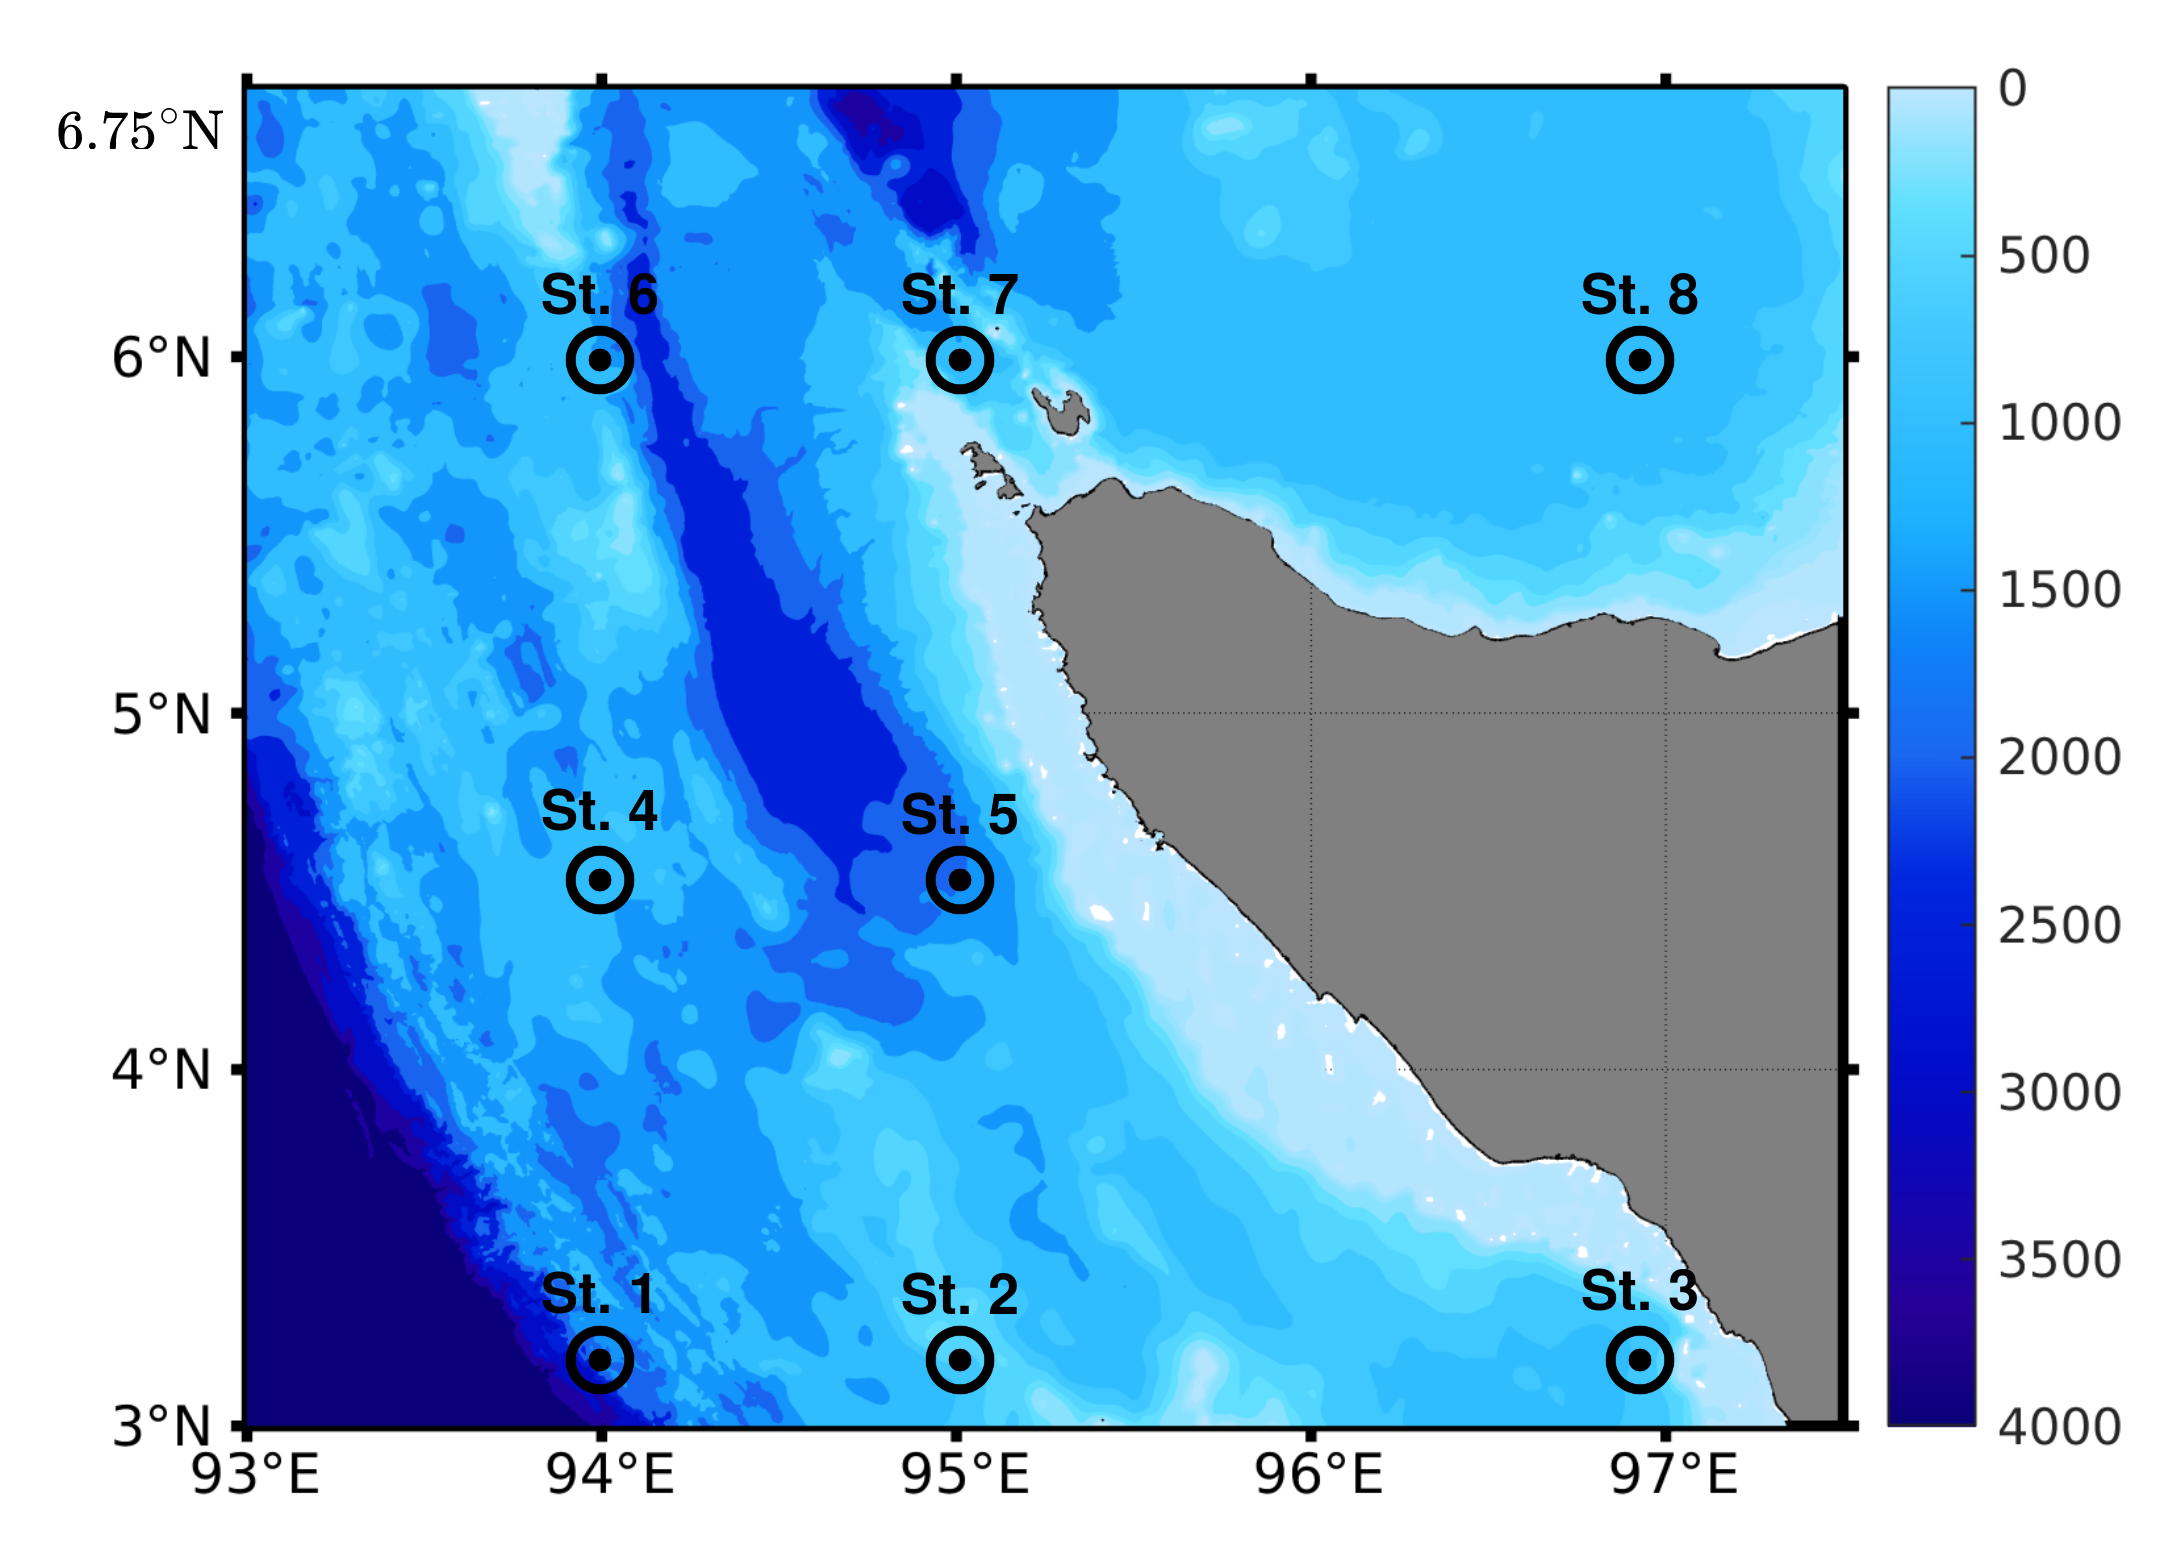
\includegraphics[width=15cm]{contents/bathymetri}
		\caption{Data batimetri domain model BoB, dicuplik dari SRTM15+}
		\label{fig:domain}
	\end{figure}
\end{spacing}
\section[Data Penelitian]{Data Penelitian}
\begin{spacing}{1.5}
\vspace{-1pc}
\subsection[Data Oseanografi]{Data Oseanografi}
	Data oseanografi yang digunakan adalah data elevasi dan arus permukaan, serta data temperature dari HYCOM (\textit{HYbrid Coordinate Ocean Model}) yang merupakan salah satu model sirkulasi laut (OGCM) yang menggunakan model numerik tiga dimensi Navier-Stokes dengan input data batimetri dari GEBCO (\textit{General Bathymetric Chart of the Oceans}), data asimilasi hidrografi laut dari NCODA (\textit{Navy Coupled Ocean Data Assimilation}) dan komponen meteorologi dari NCEP (\textit{National Centers for Environmental Prediction}) ataupun NAVGEM (\textit{The NAVy Global Environmental Model}) berupa angin, kecepatan, fluks panas, tekanan permukaan laut, presipitasi, temperature, dan kelembapan \shortcite{JosephMetzger2013}. Koordinat vertikal dalam HYCOM adalah isopiknal di lautan terbuka yang terstratifikasi dan memiliki transisi yang mulus dan dinamis serta bergantung terhadap waktu pada medan daerah pesisir yang dangkal dan pada tingkat tekanan tetap di lapisan campuran permukaan atau lautan yang tidak terstratifikasi \shortcite{chassignet2017,Park2013}. 
	\par Untuk data temperature HYCOM, data yang digunakan adalah data analisis global dengan resolusi spasial 5 menit untuk longitude dan 2.5 menit untuk latitude selama 12 bulan (Januari - Desember) tahun 2021 dan dengan ketebalan bervariasi pada bidang vertikal, yaitu 40-lapisan $(k \in [1,40])$:
	\begin{equation*}
		\begin{aligned}
			z_k = \{0.0, 2.0, 4.0, 6.0, 8.0, 10.0, 12.0, 15.0, 20.0, 25.0, 30.0, 35.0, 40.0, 45.0, 50.0, \\
			60.0, 70.0,	80.0, 90.0, 100.0, 125.0, 150.0, 200.0, 250.0, 300.0, 350.0, 400.0, 500.0, 600.0,\\
			700.0, 800.0, 900.0, 1000.0, 1250.0, 1500.0, 2000.0, 2500.0, 3000.0, 4000.0, 5000.0\} (m). \\
		\end{aligned}
	\end{equation*}
\subsection[Data Meteorologi]{Data Meteorologi}
	Data meteorologi yang digunakan adalah data reanalysis NCEP/NCAR per 6 jam \href{https://psl.noaa.gov/data/gridded/data.ncep.reanalysis.html}{(https://psl.noaa.gov/data/gridded/data.ncep.reanalysis.html)} selama 20 tahun dari tahun 2002 sampai 2021 untuk 6 parameter yaitu: 2m air temperature, 2m specific humidity, convective precipitation rate, sea level pressure, wind stress U, dan wind stress V.
\end{spacing}
\vspace{-0.5pc}
\section[Prosedur Penelitian]{Prosedur Penelitian}
\begin{spacing}{1.5}
	\begin{figure}[H]
		\centering
		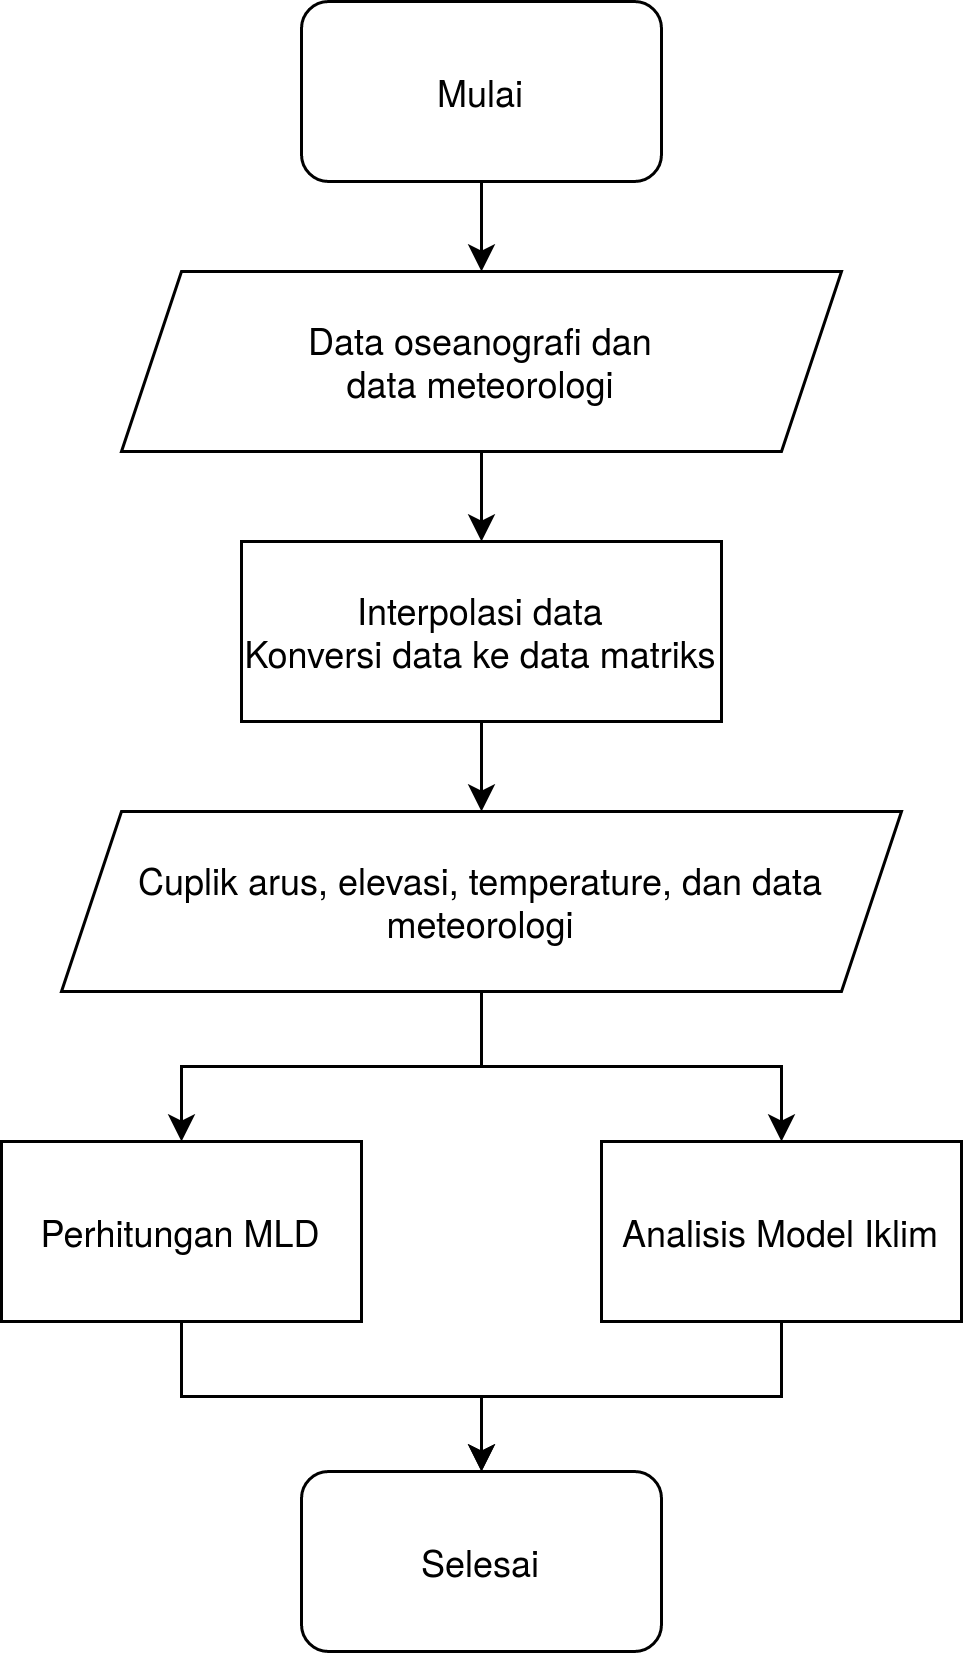
\includegraphics[width=7cm]{contents/flowchart.png}
		\caption{Diagram alir penelitian}
		\label{fig:flowchart}
	\end{figure}
	Prosedur penelitian mengikuti diagram alir pada Gambar \ref{fig:flowchart}. Data-data terkait penelitian didownload terlebih dahulu kemudian diinterpolasi untuk memenuhi data yang kosong serta untuk memperoleh resolusi spasial yang lebih detail. Selanjutnya data hasil interpolasi kemudian dibaca dan di konversi ke dalam data matriks pada MATLAB. Hasilnya adalah peta arus, elevasi, temperature, dan data meteorologi. Peta temperature kemudian diobservasi untuk menentukan kedalaman lapisan campuran selama 12 bulan. Sebagai verifikasi atas observasi kedalaman lapisan campuran, akan dilakukan analisis model iklim terhadap data meteorologi (2m air temperature, 2m specific humidity, convective precipitation rate, sea level pressure, wind stress U, dan wind stress V) selama 20 tahun dari tahun 2002 sampai 2021.
\end{spacing}